\documentclass[conference]{IEEEtran}
\usepackage{cite}
\usepackage{amsmath,amssymb,amsfonts}
\usepackage{algorithmic}
\usepackage{graphicx}
\usepackage{textcomp}
\usepackage{xcolor}
\usepackage{multirow}
\usepackage{tabularx}
%\usepackage{caption}
\usepackage{subcaption}
\usepackage{listings}
\usepackage{multicol}
\usepackage{xcolor}
\definecolor{codegreen}{rgb}{0,0.6,0}
\definecolor{codegray}{rgb}{0.5,0.5,0.5}
\definecolor{codepurple}{rgb}{0.58,0,0.82}
\definecolor{backcolour}{rgb}{0.95,0.95,0.92}
\lstdefinestyle{mystyle}{
    backgroundcolor=\color{backcolour},   
    commentstyle=\color{codegreen},
    keywordstyle=\color{magenta},
    numberstyle=\tiny\color{codegray},
    stringstyle=\color{codepurple},
    basicstyle=\ttfamily\footnotesize,
    breakatwhitespace=false,         
    breaklines=true,                 
    captionpos=b,                    
    keepspaces=true,                 
    numbers=left,                    
    numbersep=5pt,                  
    showspaces=false,                
    showstringspaces=false,
    showtabs=false,                  
    tabsize=2
}


\def\BibTeX{{\rm B\kern-.05em{\sc i\kern-.025em b}\kern-.08em
    T\kern-.1667em\lower.7ex\hbox{E}\kern-.125emX}}
\begin{document}

\title{Securing FPGA Supply Chain Through Bio-Inspired Evolutionary Strategies}


\author{\IEEEauthorblockN{Bayley King}
\IEEEauthorblockA{
\textit{Dept. of EECS} \\
\textit{University of Cincinnati}\\
Cincinnati, OH, USA \\
king2b3@mail.uc.edu}
\and
\IEEEauthorblockN{Rashmi Jha}
\IEEEauthorblockA{
\textit{Dept. of EECS} \\
\textit{University of Cincinnati}\\
Cincinnati, OH, USA \\
jhari@ucmail.uc.edu}
\and
\IEEEauthorblockN{Temesguen Kebede}
\IEEEauthorblockA{
\textit{Avionics Vulnerability} \\
\textit{Mitigation Branch} \\ 
\textit{AFRL/RYWA}\\
Dayton, OH, USA \\
temesgen.kebede.1@us.af.mil}
\and
\IEEEauthorblockN{David Kapp}
\IEEEauthorblockA{
\textit{Avionics Vulnerability} \\
\textit{Mitigation Branch} \\ 
\textit{AFRL/RYWA}\\
Dayton, OH, USA \\
david.kapp@us.af.mil}
}

\maketitle

% As a general rule, do not put math, special symbols or citations
% in the abstract or keywords.
\begin{abstract}
The increasing globalization of the Intellectual Property (IP) industry has added a new risk for designers when using 3rd party programs.
Malicous entities have more oppertunities to insert hardware trojans into these 3rd party IPs, which can often remained undetected by convential testing procedures.
Even in the case where these trojans could be detected from a full testing suite, the time associated with running the full suite could be inpheasable or the full testing suite might not be available to the designer.
This work proposes the use of an Evolutionary Strategy (ES) which only needs partial test cases to remove hardare trojans from infect 3rd party Hardware Design Language (HDL) IPs.
We applied this system to infected circuits, and showed that fault injecting hardware trojans can be removed without removing the desired logical functionality of the original un-infected program.
The synthesized designs of the evolved programs are then tested in Vivado and run on a Field Programmable Gate Array (FPGA), where the evolved code showed no additional overhead comapred to the original unifected code.
We then conclude with some future works in the area of partial test case generation on larger circuits containing more complex hardware trojans.
\end{abstract}

% Note that keywords are not normally used for peerreview papers.

%%%%%%%%%%%%%%%%%%%%%%%%%%%%%%%%%%%%%%%%%%%%%%%%%%%%%%%%%%%%%%%%%%%%%%%%%%%%%%%%%%%%%%%%%%%%%%%%%%%%%%%


\section{INTRODUCTION}
\par The FPGA supply chain has become increasingly vulnerable to attacks, not only in the physical device supply chain, but in the IP that is run on the boards.
Little work has been completed to add trust to the supply chain of 3rd party Hardware Design Language (HDL) programs, which is of concern due to the frequent use of 3rd party software.
A malicious agent could hide a hardware trojan inside of a 3rd party Intellectual Property (IP) that is even undetacable from contemporary testing methods\cite{}.
Work has been done to try and combat this \cite{}, but there are still many challenges facing the field.
One of the key challenges is the availability of exhaustive testing suites for designers to use when checking the 3rd party IP.

\par In this work we report a novel bio-inspired appraoch for repairing and securing 3rd party HDL IPs by using an ES. 
We tested various mutation schemes across different circuit types and report on the success rate of each evolution, statistics realated to the evolutionary process, and qauntitative data related to the evolved programs.
Our approach showed that evolutinary strategies can remove combinational hardware trojans with exhasutive testing suites, and even with partial testing suites. 
The succesfully evolved circuits added no extra overhead to the sythnesized design, and performed the desired logical tasks.
Remainder of this paper is structured as: section (1) discussing our threat model and overall mitigation approach, section (2) gives a brief overview of evoluionary computing, section (3) talks about implementation, section (4) results and discussions on our test cases, and finally section(5) discusses the conclusions. 
We believe that this approach provides a promising route to add an extra layer of security to the supply chain of 3rd party HDL IPs to protect against malicous entities.

%%%%%%%%%%%%%%%%%%%%%%%%%%%%%%%%%%%%%%%%%%%%%%%%%%%%%%%%%%%%%%%%%%%%%%%%%%%%%%%%%%%%%%%%%%%%%%%%%%%%%%%

\section{Threat Model and Mitigation}
\par With the increasing popularity in use of 3rd party HDL IPs, malicious entities have an even larger oppertunity to inject hardware trojans in the FPGA supply chain.
These trojans can often be undetectable by conventual testing schemes CITE.
Our threat model assumes that a malicous entity inserted a trojan into the program, and it remains undetected.
Our proposed mitigation is to use an ES to evolve the program to either repair the program by removing the trojan, or scrambling the trojan to a point where it no longer performs its initial task.
Figure \ref{fig:network} shows our proposed mitigation to this threat model.

\begin{figure}[t]
    \centering
    \includegraphics[width=0.4\textwidth]{Images/host_system_info.PNG}
    \caption{System flowchart information} % I have no clue what to call this......
    % NEED TO FIX. ADD BACK ORIGINAL PARTS AND SCALE DOWN
    \label{fig:network}
\end{figure}

A successful evolution would be where the evolved code performs all the desired logical tasks and is diverse from the parent code.
This diversity is measured by looking at the edit distance between the two programs, more of this will be discussed in section \ref{net:fitness}.
Once the program is evolved, we compare the two synthesized designs of the original and evolved programs. 
A properly evolved program should synthesize the same as its un-infected parent, or would synthesize a clean version of the 3rd party IP no longer infected by the hardware trojan.
To gain achieve this mitigation plan, we researched hardware trojans on FPGA and bio-inspired approaches within the field of hardware security.

\subsection{Hardware Trojans on FPGA}
\label{wbd:trojans}
\par Shakya et. al\cite{benchmarking of hardware trojans and malicous} identified that trojans on FPGAs can either be IP-dependant or IP-independant, in our work we will focus on IP-dependant trojans.
These trojans can corrupt Look Up Table (LUT) values, load incorrect values into memory or modify configuried designs. 
The activations for these trojans can be the same as silicon based trojans (always-on, triggered, etc) but FPGAs offer a new activation type\cite{novel feature extraction strategy for hardware torjan detection, benchmarking of hardware trojans and malicous}.
The trojan activation on the FPGA can also be triggered by monitoring specific LUTs on the board, that once triggered either cause a malfunction or leak IP.
The malfunction could be as simple as corrupting data, to damaging the FPGA device.

Model checking and automatic test pattern generation (ATPG) are commons ways to try and detect these hardware trojans\cite{hardware trojan detection using atpg, toward fpga securty it iot, novel feature extraction strategy for hardware torjan detection} but most works focus on the rtl representation of the program, not the HDL code itself.
The detection of trojans is widely discussed in literature, but little has been said in response to malicious behavior. 

\subsection{Bio-inspired approaches in hardware security
\label{wbd:ea}
\par Using evoluionary computing to add a layer of trust is not a new conecpt in the field of hardware security field. 
Various algorithms raning from genetic algorithms{ping yu, collins2019evolvable}, simulated anleaing{hereboy}, particle swarm optimization{ping yu,} and genetic programming (GP){popp montana gassner, koza, gordon bentley}
These works usually start with randomly generated programs, and evolve them to create a valid solution.
Generating a new circuit from scratch would require a full testing suite for trainning, which is not always available to designers. 
Larchev and Lohn CITE used evolutionary techniques to repair faults on FPGA by evolving LUTs and their conenctions.
Their population consisted of a set of randomly generated circuits, and copies of the original circuit. 
Few proposed solutions take the avialibility of full testing suites into consideration, which leaves a vulnerability in the supply chain for 3rd party IPs.

%%%%%%%%%%%%%%%%%%%%%%%%%%%%%%%%%%%%%%%%%%%%%%%%%%%%%%%%%%%%%%%%%%%%%%%%%%%%%%%%%%%%%%%%%%%%%%%%%%%%%%%
\section{Evolutionary Algorithms}
\label{ea:intro}
\par An Evolutionary Algorithm (EA) is a bio-inspired approach to solve computational problems across various topics within the field of computer science. 
EAs take inspiration from the process of evolution through a population from the use of selection, mutation and reproduction. %https://en.wikipedia.org/wiki/Evolutionary_algorithm 
The most common version of EAs are Genetic Algorithms (GA), which are a metaheuristic approaches to optimize some fitness function by simulating natural selection. 
A population of individuals are tested on some fitness, and are then selected to mutate and re-populate the next generation of individuals. 
Many other variants of EAs exist, but the core features of them follow the process of a standard evolutionary algorithm. 
\subsection{Standard Evolutionary Algorithm}
\label{ea:standard_ea}
\par A standard evolutionary algorithm simulates natural selection by evolving populations of individuals to meet a certain goal over a set of generations. 
In a generation, a group of parents are selected from the full population to seed the next generation.
These parents under go mutation and or recombination to fill a child population, which then undergoes a selection procedure to decide who will join the population into the next generation. 
There are five main functions to a standard EA: the population function, the fitness function, the parent selection function, the variation function and the survivor selection function
% some double figure showing crossover and a tree encoded individual

\subsubsection{Population Function}
\label{ea:population_function}
\par The population function determines how individuals are represented in the evolutionary process and how many individuals exist in the population. 
The population is a multiset of these individuals, meaning that multiple copies of the same individual can exist in a given population. 
Each individual represents a possible solutions to some problem, the individual is referred to as a phenotype in the problem space and the encoding of these individuals inside the EA is then called their genotype.
Encoding schemes vary greatly (floating point values, binary strings, sequences) with each representation creating a different genotype space for the EA to search for valid individuals.
After the individual representation is selected, then some parameter $n$ is set to be the number of individuals in the population. 
% CITE

\subsubsection{Fitness Function}
\label{ea:fitness_function}
\par The fitness function is some way to measure how well an individual performs its desired task(s). 
This can be done by either calculation (evaluating the direct encoding) or by some performance metric.
In some cases the direct encoding genotype of the individual are used in the fitness calculation, other times the genotype must then me mapped to some expression to calculate fitness.
For example if the individual is a circuit, then fitness could measuring how well the circuit performs a testing suite.
% cite some Kashtan works, look under complex systems reading under evolvablilty modulatiry

\subsubsection{Parent Selection}
\label{ea:parent_selection}
\par The parent selection function decides which individuals in the current population will be seeded to repopulate and the next generation of individuals. 
The parent selection function mimics deciding who survives natural selection, and isn't always as simple as just selecting the most fit individuals. 
An individual with a higher fitness has a better chance at being selected, but a purely greedy approach that only selects the best performing individuals is rarely used due to the evolution getting stuck in a local optimum.

\par There are three major subsets of parent selection algorithms: elitist, non-elitist, and hybrid. 
An elitist approach would be where the fittest individual(s) are always selected, a non-elitist approach would be some random selection, and hybrid would be some combination of the two. 
Since the searching space is often very rough, greedy and elitist selection functions won't traverse this space as well and a function that combines elitist and non-elitist approaches\cite{eiben2003introduction}.
Stochastic approaches have been used that select an individual with a probability based on one's fitness value, often called a roulette wheel selection, but knowledge of the entire population is needed to generate these fitness scores.
A very common selection function is a tournament style approach where $x$ number of individuals are chosen from the population, then the best performing individual from the set of $x$ individuals is selected to join the parent population. 

\subsubsection{Variation Function}
\label{ea:variation}
\par The variation function, or mutation function, is used to generate new individuals by varying the genome of members of the parent population. 
This is done through mutation, slightly modifying the individual, and recombination (crossover), merging two parent genotypes into one or more genotypes. 
Recombination mimics reproduction in the biological world, where the child/children individual's genotype is a combination of their parent's genotype.
Mutation and recombination are stochastic operators, both varying greatly in implementation across the many encoding types.
The variation function is used to generated similar candidates to the parent population, that might perform better or worse than their parents, in the hope that the slight variations will help find more optimal solutions.

\subsubsection{Survivor Selection}
\label{ea:survivor_selection}
\par Once the individuals from the parent population have undergone mutation and recombination, they will be used seed the next generation.
In theory, the mechanisms used in section \ref{ea:parent_selection} could also be used to select the survivors, but various selection operations aimed specifically at survivor selection have been used throughout literature.
The types of survivor selection strategies are age-based and fitness-based replacement, then a combination of the two. 
An age-based selection would look at only the number of generations each individual have survived, instead of fitness, similar to the operation of a FIFO.

\par Some fitness-based schemes were described in section \ref{ea:parent_selection}, and function mostly the same for survivor selection except in the number of individuals selected.
Often the size of the parent population, child population and survivor population are different.
A large parent population can remove fitness-based selection pressure, but can lead to premature convergence to a local optimal solution. 
Using a separate fitness-based selection scheme for both the parents and the survivors can then limit the selection pressure from the varying sizes in populations.

\subsection{Genetic Programming}
\par A variation on the EA is Genetic Programming (GP) which is a heuristic application in which a population of unfit programs are evolved. 
Instead of thinking of GP as an optimization problem, which is a normal assumption for EAs, we think of GP as an approach to generate a viable solution to a problem, similar to machine learning\cite{eiben2003introduction}.
GP still follows the same steps of a standard EA, but a tree structure is used to represent the genotype and an individual has a chance to partake in either mutation or recombination, not both. 
A common case is to represent each individual code as an abstract syntax tree (AST), which is an abstraction of the source code of a program.
The trees are often generated randomly between a minimum and maximum depth of some set of functions.
Koza\cite{koza1992genetic} pioneered work on genetic programming, and has suggested the sole use of recombination during genetic programming without the possibility of mutation.

\par The largest overhead in the genetic programming is normally the fitness function, since the time taken to compute the fitness function increases with an increase in the size of the population and the complexity of the problem space.
The time complexity of a fitness function for a circuit is $o(2^n)$ with $n$ being the number of inputs, if exhaustive testing is used to score the fitness of the circuit. 
Work has been done looking at introducing modularity into fitness functions to help speed up the convergence of these evolutionary processes, while also decreasing the time needed to reach these converged solutions. % cite here boy, kashtan, etc. Lots to cite here

\subsection{Evolutionary Strategies}
\label{ea:es}
An Evolutionary Strategy (ES) were first proposed in the 1960s by Rechenberg and Schwefel to investigate evolutionary approaches to shape optimization\cite{beyer2002evolution}.
The earliest forms of ESs featured populations of two individuals, often called $1+1$ ES, but various other forms exist like the $\mu,\lambda$ and the $\mu,\lambda$ where $\mu$ is the size of the population and $\lambda$ is the parent population size.
ES follow the EA more closely than GP, and normally just utilizes different selection functions, since the population sizes are often smaller.
In most cases, a steady state population is used where the parent, children and survivor populations are all the same size.

\par In an ES with a small population, recombination becomes less useful compared to mutation, and even becomes impossible when you have a population size of 1.
Instead, mutation is the sole factor used for variation during the evolutionary process.
The comparison between an EA and an ES can be seen in Figure \ref{fig:ea_vs_es}.

\begin{figure}[t]
    \centering
     \begin{subfigure}[b]{0.2\textwidth}
         \centering
         \includegraphics[width=\textwidth]{Images/host_paper-ea.jpg}
         \caption{EA Flowchart}
         \label{fig:ea_flowchart}
     \end{subfigure}
     \hfill
     \begin{subfigure}[b]{0.2\textwidth}
         \centering
         \includegraphics[width=\textwidth]{Images/host_paper-es.jpg}
         \caption{ES Flowchart}
         \label{fig:es_flowcahrt}
     \end{subfigure}
     \caption{Comparison of evolutionary process for a standard EA and a (1,1) ES}
     \label{fig:ea_vs_es}
\end{figure}

\subsection{HereBOY}
\label{ea:hereboy}
\par The HereBOY algorithm is a positive hill climber variant of an evolutionary algorithm, which utilizes the idea of having a population size of one circuit\cite{levi2000hereboy}. 
In this work Levi considers a circuit as the FPGA bitstream representation, which is just a string of 0s and 1s. 
The EA will flip bits in the bitstream (mutation), compile and test the new circuit (fitness function) and then compare the fitness of this new circuit to the old circuit (selection).
If this new mutated circuit had a higher fitness than its parent, then the parent dies off and the child survives to the new generation.
If the parent had a higher fitness, than the mutations are reversed and the child is discarded to allow the parent to survive to the next generation.
This approach is highly susceptible to getting stuck in a local optimal, especially with a more complex problem space.
We took interest in the mutation scheme, especially the adaptive mutation rate in our network, and wanted to test a purely software variation of this EA against other EAs.

%%%%%%%%%%%%%%%%%%%%%%%%%%%%%%%%%%%%%%%%%%%%%%%%%%%%%%%%%%%%%%%%%%%%%%%%%%%%%%%%%%%%%%%%%%%%%%%%%%%%%%%

\section{Our network}
\label{net:intro}
%%% Still needs a name %%%  Probably something using ES in it
\par Our threat model follows the depiction in figure \ref{fig:supply_chain} where some malicious entity infects a 3rd party HDL with a trojan.
A designer won't always have access to an exhaustive testing suite to fully test a 3rd party code, but even if they had access to the full testing suite not all hardware trojans can be detected using a full testing suite.
Some trojans have sequential triggers that either wait for sequential keys by tapping internal wires, or have "time-bomb" triggers that use counters to inject faults onto a wire. 
Trojans like these are discussed more fully in section \ref{wbd:trojans}.
We make an assumption that the 3rd party HDL contains a trojan that is undetectable by standard testing measures and that the designer only has access to a partial testing suite.
The designer could then evolve this un-trusted 3rd party HDL IP with our ES, to create a diverse variant that was structurally different but still passed the required logical functions. 

\par To solve these issues, we built our own custom genetic programming framework to test if evolutionary strategies would be useful to remove hardware trojans from HDLs using partial test cases. 
Although this network evolves a program using evolutionary means we don't call this network a genetic programming due to some key differences in the population, fitness, mutation and selection functions. 
We still refer to this as an evolutionary strategy that uses a tree structure as its genotype.
The goal of the evolution is to generate a new individual that passes a full exhaustive testing suite and has removed the trojan, or modified it so that the trojan no longer serves any malicious functions. 


\subsection{Population Function}
\label{net:population}
\par We chose to use HDL ASTs to represent our individual's genotype, which is made up of structural logical gates (AND, OR, NOT, XOR, NAND, etc) and input signals. 
Figure \ref{fig:2-1_mux} show the AST of a simple 2-1 Multiplexer (MUX) represented by our choice in genotype.
We then chose to use a (1,1) ES, meaning that our population is of size 1 and that the child individual always replaces the parent individual. 
This initial genotype of the individual is the presumably trojan infected HDL. 
Since we don't have access to an exhaustive testing suite, our initial individual needs to already perform some of the desired logical functionality and can not be a randomly generated individual.

\begin{figure}[htb]
    \centering
    \subfloat{
        \includegraphics[width=0.23\textwidth,keepaspectratio]{Images/2-1mux.png}
    }
    \subfloat{
        \includegraphics[width=0.23\textwidth,keepaspectratio]{Images/normal_2-1_mux.png}
    }
    \caption{AST and gate level circuit design of a 2-1 Multiplexer}
    \label{fig:2-1_mux}
\end{figure}


\subsection{Fitness Function}
\label{net:fitness}
\par In normal GP, the actual logical functionality divided expected logical functionality acts as the fitness function, giving an individual a score in the range $[0,1]$ which we will call $F_i$.
We are assuming that the infected circuit already has a fitness value of 1, meaning that the actual and expected logical functionalities are the same at the start of the evolution.
This would normally trigger the exit conditions for the ES, but we haven't met our goal of removing the hardware trojan.
To counter this, we propose the use of a second fitness function to measure the similarity of the original circuit and the current circuit. 
We want our evolved individual to not only be structurally diverse from the original HDL, but perform the same desired logical functionality, giving us two measurable fitnesses; similarity, and logical functionality.
Our hypothesis is that a structurally diverse evolved circuit should nullify the trojan, and render it useless.

\par We chose to use the the levenshtein (edit) distance between two trees to measure the similarity of the two circuits since it is a well studied method to compare two tree structures\cite{xu2015algorithm,zhang1989simple,zhang1992editing}.
We rate each circuit with a normalized value, $S_i$, in the range of $[0,1]$.
\begin{equation}
    S_i = Lev(Ind_0,Ind_i) / max(len(Ind_0),len(Ind_i))
\end{equation}
The original circuit is called $Ind_0$ and the current circuit (in the $ith$ generation) is called $Ind_i$.
The levenshtein distance is now normalized to the length of the longest circuit out of the original and current individual.
This value of $S_i$ can then be used as a second fitness value during the evolution along side $F_i$.

\par Kashtan and Alon proposed the use of multiple fitness functions to include modularity in their networks by showing their network multiple goals during the evolution\cite{kashtan2005spontaneous}.
Although we are not using various logical functionalities as our multiple fitness functions, we mimicking the conclusions they reached where including additional behaviors can lead to more diverse and robust solutions.
We chose to vary the weight of $S_i$ and $F_i$ over the evolutionary process with structural fitness weighted of higher importance in the initial stages of evolution, to drive structural change, but gradually increasing the importance of the logical fitness until a floor value is met for $S_i$.
The weights of $S_i$ and $F_i$ can be thought of as scalars to sum the logical and structural fitness the individual currently posses into a single fitness score.
The change in weights over the number of generations can be seen in Figure \ref{fig:fitness_plots}.
The sum of the weights of $S_i$ and $F_i$ at any given generation is always 1, meaning that our individual still has a single measurable fitness in the range of $[0,1]$. 
Upon a successful evolution, the new individual would not only perform the desired logical tasks but also be above a minimum normalized levenshtein distance from the original HDL.


%%%%%% RE DO THIS PLOT WITH GENERATIONS ON THE X AXIS %%%%%%%%
\begin{figure}[t]
    \centering
    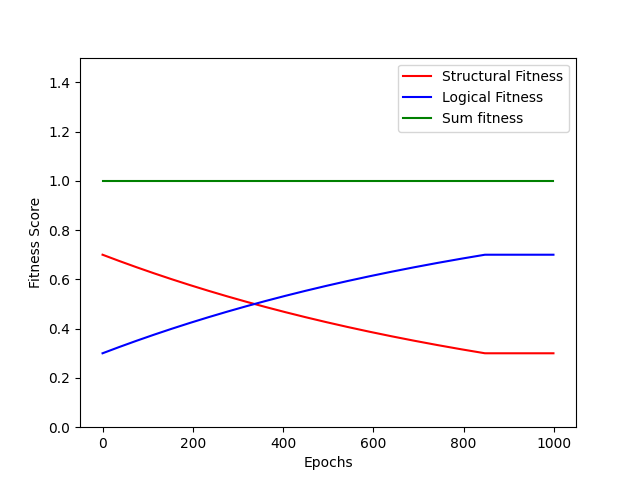
\includegraphics[width=0.5\textwidth]{Images/output_plots.png}
    \caption{Weighting of Logical Fitness ($F_i$) and the Structural Fitness ($S_i$)}
    \label{fig:fitness_plots}
\end{figure}


\subsection{Variation Function}
\label{net:variation}
\par As mentioned in section \ref{ea:es}, it is impossible to preform recombination on a (1,1) ES due to its population size.
Our network only uses mutation to preform variations.
There are currently three types of mutations that can be performed for our evolutionary strategy. 
Since our population consists of a single individual, we cannot perform a normal recombination of individuals to generate a new individual.
Although, we can perform random mutations on the individual similar to a normal genetic algorithm, where we could add nodes, remove nodes and mutate nodes.
\subsubsection{Add Node}
A leaf node is changed into an operation node with two randomly generated children. 
\subsubsection{Remove Node}
A node and all of its children are removed from the tree, with a random leaf node inserted in its place. 
Only leaf branches can currently be selected, IE nodes with only two children. 
\subsubsection{Mutate Node}
A node's value is randomly changed to another of the same type. A node that is an input will change to another input, then a node that is an operation will change to another operation. 

\subsection{Selection Function}
\label{net:selection}
\par Since we are using a (1,1) ES, we don't need to select which parent will seed the next generation, or which child survives into the next generation.
Instead, we select which mutation to make in the current generation, and where in the tree that mutation will take place.
In our system, we implemented three different selection functions to select these mutations: the Software HereBOY, exhaustive mutation checking, and stochastic mutations.
\subsubsection{Software Hereboy}
\par This approach is a positive hill climbing method, which is similar to the HereBOY hardware evolutionary algorithm described in section \ref{ea:hereboy}.
There is some mutation rate defined by
\begin{equation}
    \alpha = 0.1*Len(AST)
\end{equation}
\begin{equation}
    \beta = (MaxScore – MaxCurrentScore)/MaxScore
\end{equation}
\begin{equation}
    Number Of Mutations = \alpha * \beta
\end{equation}
A number of mutations are then performed on the individual, and its new fitness is calculated.
If this new individual has a higher fitness than its previous self, then the mutation(s) are accepted and carry over to the new individual.
If the mutation(s) cause a decrease in fitness, then they are discarded and the previous individual moves onto the new generation.
\subsubsection{Exhaustive}
\par Every possible mutation is performed on the current individual, and their resulting offspring is added to a parent population. 
The highest performing individual is then selected to survive to the child generation, giving us another positive hill climbing approach, expect in this case we are guaranteed the steepest possible ascent.
Although not necessarily in nature, it is a good metric to compare against since it resembles a brute force approach.
\subsubsection{Stochastic}
\par Each possible mutation type (add node, remove node, and mutate node) are given a weighted chance to be selected, much like the roulette wheel selection function in a standard genetic algorithm.
We very early found out that given our low population size of one individual, that we couldn't just rely on purely random mutations to generate a valid solution. 
We needed the highest chance that the selected mutation would cause an higher increase in fitness. 
To do this, we added a new mutation type which we call the exhaustive node mutation check, where every possible node mutation is added to a parent population and the highest performing individual is then selected. 
This new mutation is weighted higher than the three mentioned in the previous subsection, along with the chance that no mutation is performed on the individual. 

\subsection{AST to Verilog}
\par Once the evolved AST has passed its exit conditions, it is ready to be transformed back into an HDL program.
Modern day HDL compilers, like Vivado, can generate bitstreams from verilog/vhdl across different program styles.
Behavioral code is a popular choice, due to its similarity to c-based programming languages.
The final synthesized design is independant of the coding style used, so the main benefit for the different HDL coding sytles is readability for the user.
We created a system to translate our evolved ASTs into structural verilog, since strcutrual verilog is similar to the AST representation we chose for our programs.
Each gate, input and output are defined with a label, where the labels serve are inputs to other gates. 
Our script starts by making a dictonary of every node (gate) in the AST and then links its branches by their unique label. 
Once the labels have been linked, a simple code generation is performed to write the structural verilog into a file. 
This file is then the HDL representation of the evolved circuit, which can be compiled just like any other HDL file.

%%%%%%%%%%%%%%%%%%%%%%%%%%%%%%%%%%%%%%%%%%%%%%%%%%%%%%%%%%%%%%%%%%%%%%%%%%%%%%%%%%%%%%%%%%%%%%%%%%%%%%%

\section{METHODOLOGY}
\par Although the main goal that was outline in previous sections was to evolve an presumably infected HDL with partial test cases, we wanted to verify the network by running other tests.
Due to the stochastic nature of these tests, every simulation was ran 20 times so their results could be averaged.
To first verify that the ES can perform GP, we allow the following tests to use the exhaustive testing suite during the evolutionary process, but later tests then limited the available testing suite to match our original threat model.
The goal of the tests would be to verify the usability of this ES across different evolutionary goals.
Three testing types were created; random start to working logic, variant creation and trojan removal.

\subsection{Start Types}

\subsubsection{Random to working logic}
\par This mimics a normal genetic programming simulation where the starting circuit is a piece of random logic that is evolved to perform some task.
In our case, this task is some logical functionality that is predefined, like a 2-1 MUX or some combinational logic.
This test verifies that our ES can performing GP in the simplest case. 

\subsubsection{Variant Creation}
\par The starting circuit already performs the desired logic tests, but a different version of the circuit is desired at the end of the evolution.
This was inspired by Collins et. al\cite{collins2019evolvable} where variant circuits were generated to add an extra layer of security to hardware designs.
At the end of the evolutionary process, the evolved circuit should perform the same logical function as the original circuit while have a different and diverse genotype. 
We set some minimum normalized edit distance, and for a successful evolutionary process the end circuit must be at least this minimum distance away from the original circuit and still have the desired logical functionality.

\subsubsection{Trojan Removal}
\par A combinational trojan is inserted onto a random wire in the circuit, which injects a fault whenever triggered. 
This trigger is some random combination of inputs, that range in size of $N-1$ to $1$ for a circuit with $N$ total inputs.
These randomly selected inputs feed into an AND gate whose output is fed into an XOR gate with the randomly selected wire from the circuit. 
Whenever the input sequence is triggered the randomly selected wire's result is flipped, since the output from the AND gate does goes high which turns the XOR gate into inverter for the other signal. 
Although a combinational trojan can take many different shapes, the we chose to create them in the simple implementation seen in Figure \ref{fig:comb_trojan}.
This type of trojan is not only simple to implement, but simple to verify both pre/post evolution. 
Since a fault is injected from a given input sequence, the effectiveness of this trojan can be tested by inputting the required sequence and monitoring if a fault was generated.
In the case of a successful evolution, the combinational input sequence for the circuit will no longer inject a fault into the circuit.

\begin{figure}[t]
    \centering
    \includegraphics[width=0.4\textwidth]{Images/combt_trojan.jpg}
    \caption{Simple Fault Injecting Combinational Trojan}
    \label{fig:comb_trojan}
\end{figure}

\subsection{Partial Test Cases}
\par When a designer uses a 3rd party IP, a full testing suite might not be available to them or it could be unfathomable to run a full testing suite prior to the usage of the code.
We selected random tests from the exhaustive testing suite, and then rant the previously mentioned tests to verify if partial test cases could still allow for successful evolution's. 
It is important to note that to consider an evolution successful, the final circuit must pass the full exhaustive testing suite.
This is checked after the exit conditions are met for the ES just for verification purposes.

\par In these initial tests, we selected a set number of tests in the exhaustive testing suite randomly to represent the partial test cases.
Our reasoning is that a random selection would offer the lowest chance of success due to the random code coverage this partial suite offered.
We assume that the designer would have a partial testing suite which offered higher code coverage than random selection, so one could expect that the results of this test would improve along with a better test case generation. 

\subsection{Scalability}
\par One of the key criticisms of GP is its poor scalability to larger circuits. % CITE HERE
The problem spaces become too large and complex for the heuristic approach to find valid solutions in a reasonable time.
We wanted to measure the speedup of our ES in these more complex and larger spaces, so we created various sizes of combinational logic and measured the success rate as the circuits increased. 
We also varied the number of inputs to increase the complexity of the problem space, since the number of inputs to a circuit directly effects the size of its logical fitness space.

%%%%%%%%%%%%%%%%%%%%%%%%%%%%%%%%%%%%%%%%%%%%%%%%%%%%%%%%%%%%%%%%%%%%%%%%%%%%%%%%%%%%%%%%%%%%%%%%%%%%%%%

\section{RESULTS AND DISCUSSIONS}
\par The stochastic mutation rates and parameters were used for all of the following tests can be seen in Table \ref{tbl:partial_params}.
\begin{table}
\centering
    \begin{tabular}[\textwidth]{||p{1cm}|p{1cm}|p{1cm}|p{1cm}|p{1cm}|p{1cm}||}
         \hline
         Runs & Max Gens & Best Node & Random Node & Add Node & Rem Node \\ [0.5ex] 
         \hline\hline
         20 & 4000 & 50\% & 30\% & 10\% & 10\%\\ 
         \hline
    \end{tabular}
    \caption{Testing Parameters}
    \label{tbl:partial_params}
\end{table}


\subsection{Network verification}
\par The results shown in Table \ref{tbl:basic_results} are the outcomes of the verification tests to make sure the ES could solve basic evolutionary problems. 
The three different starting types were tested with each selection scheme described in section \ref{net:selection}.
A success occurs when the evolved circuit performs all the desired logical functions and is at least the minimal normalized edit distance from the original circuit.
Our ES more than showed that it was capable of performing GP, with most tests yielding a 100\% success rate. 
Each evolved circuit had a final normalized edit distance above 1, which means that for an AST with length 20 had over 20 edits needed between itself and the original AST.
\par The random start type is the most similar to a standard GP, due to the initial randomness in the search space, and in turn yielded the most diverse evolved circuits.
The variant start type took the longest out of the three on average to run, which we believe is due to the high initial logical fitness but low initial structural fitness. 
The combinational trojan start type had a high success rate while still yielding diverse individuals.
\par The more interesting results from this test is looking at the differences between the selection schemes.
The software HereBOY selection scheme performed the worst, because the ES got stuck in a local optimum in 60\% of the tests and was unable to escape with just a single searcher.
This result was to be expected since the approach is a positive hill climber searcher.
The exhaustive checking unsurprisingly worked well, and extremely fast needing only ~2 generations to meet the necessary exit conditions. 
This approach again is a positive hill climber, but it is a guaranteed maximum positive climb since it implements the mutation that will cause the highest overall increase in fitness.
While not being necessarily biologically feasible in practice, and is more of a brute force search, this scheme served as a good benchmark for future tests.
The stochastic scheme mirrors mutations seen in EAs more than the others, but still gave high performance across all three start types. 
Although the end circuit was less diverse than the other two schemes, the end circuit was still well vastly different than the starting circuit and in each case the fault injecting trojan was rendered useless.
This means that the trojan was either evolved out from the circuit and/or its trigger was nullified to no longer inject a fault.
\begin{table}
    \begin{tabular}{|| c | c | c | c | c||}
         \hline
         Algorithm & Start Type & Success & Epochs & Similarity \\ [0.5ex] 
         \hline\hline
         \hline
         \multirow{3}{5em}{HereBoy} 
         & Random  & 100\% & 2142 & 1.27 \\ 
         & Variant & 60\% & 3294.8 & 1.37 \\
         & Comb Trojan & 60\% & 3286.4 & 1.27 \\
         \hline  
         \multirow{3}{5em}{Exhaustive Checking} 
         & Random  & 100\% & 1.4 & 1.42\\ 
         & Variant & 100\% & 2.2 & 1.44 \\
         & Comb Trojan & 100\% & 2.2 & 1.09 \\
         \hline  
         \multirow{3}{5em}{Stochastic} 
         & Random  & 100\% & 93.6 & 1.18 \\ 
         & Variant & 100\% & 432.2 & 1.00 \\
         & Comb Trojan & 100\% & 17.4 & 1.09 \\
        \hline
    \end{tabular}
    \caption{Network verification}
    \label{tbl:basic_results}
\end{table}

\subsection{Scalability with Comb Logic}
\par PLOTS SOON TO COME
\par Plot the (convergence, size, num epochs, similarity) vs (circuit size/inputs)

\subsection{Partial Test Cases}
\par We now selected a random portion of the exhaustive testing suite to create a partial testing suite to be used during the evolutionary process.
This partial scheme has random code coverage over the circuit, and was different in every simulation.
Only the stochastic mutation scheme was used for these tests, while a variable amount of partial test cases are now tested across all three start types. 
A successful evolution will be the minimum normalized edit distance from the original and will pass the full exhaustive testing suite after the ES has met its exit conditions. 
This again means that the full testing suite is not used during the evolution at any point, it is only used for verification after the fact. 
\par The results were not as strong when only partial test cases were used for the evolution, but the ES was still able to make viable solutions is some cases.
The strongest results were when 80\% of the exhaustive test cases were used as partial test cases, with the weakest results taking place when 60\% of the exhaustive suite was used.
This is to be expected, the higher percentage of tests gave a much higher code coverage which in term lead to more successful evolutions.
One can expect that using a code coverage algorithm to generate the partial test cases would increase the success chance, since the random selection would be considered the poorest code coverage tool.
\par An interesting result was that the average number of generations remained quite low.
Although the final circuit didn't always pass the exhaustive testing suite after the exit conditions were met, the process was substantially quicker than the tests seen in Table \ref{tbl:basic_results}.
The similarity scores remained just as high, if not higher than the tests with exhaustive test cases available. 
Although the results were not as definitive as the tests with exhaustive test cases, they were still promising since much better partial test cases suites can be developed with code coverage algorithms.
\begin{table}
    \begin{tabular}[\textwidth]{||p{0.8cm}|p{2.2cm}|p{1cm}|p{1cm}|p{1cm}||}
         \hline
         Test Cases & Start Type & Success & Epochs & Similarity \\ [0.5ex] 
         \hline\hline
         \hline
         \multirow{4}{5em}{80\%} 
         & Random  & 55\% & 28.8 & 2.67 \\  
         & Variant & 60\% & 49.2 & 1.07 \\ 
         & Comb Trojan & 50\% & 58.65 & 1.08 \\
         \hline  
         \multirow{4}{5em}{70\%} 
         & Random  & 20\% & 24.8 & 2.58 \\ 
         & Variant & 40\% & 60.8 & 1.04 \\ 
         & Comb Trojan & 35\% & 24.3 & 1.03 \\ 
         \hline  
         \multirow{4}{5em}{60\%} 
         & Random  & 25\% & 9.25 & 2.64 \\  
         & Variant & 20\% & 53.9 & 1.05 \\ 
         & Comb Trojan & 20\% & 42.8 & 1.05 \\ 
         \hline  
    \end{tabular}
    \caption{Results from the partial testing suite used for evolution and exit conditions}
    \label{tbl:partial_results}
\end{table}

\par We wanted to see if still using the same random partial test case suite to measure fitness during the evolution, but allowing the ES to check the exhaustive testing suite for exit conditions would yield different results. 
This scenario could be applied to a case where using the exhaustive testing suite, or a testing suite with a very high code coverage, was available to the designer but they wanted to cut back on the overhead associated with the ES.
Since the partial testing suite is being used during the evolution, the amount of computation time is decreased since fitness calculations take less time in each generation. 
The exhaustive suite is only tested on the circuit when the circuit eventually passes the partial suite fully, or has a logical fitness score of 1 during the evolution.
Results for this are shown in Table \ref{tbl:full}.

\begin{table}
    \begin{tabular}[\textwidth]{||p{0.8cm}|p{2.2cm}|p{1cm}|p{1cm}|p{1cm}||}
         \hline
         Test Cases & Start Type & Success Rate & Epochs & Similarity \\ [0.5ex] 
         \hline\hline
         \hline
         \multirow{4}{5em}{80\%} 
         % all updated
         & Random  & 100\% & 24.0 & 2.79 \\  
         & Variant & 100\% & 386 & 1.17 \\
         & Comb Trojan & 66.67\% & 386 & 1.29 \\
         \hline  
         \multirow{4}{5em}{70\%} 
         & Random  & 100\% & 85.3 & 2.47 \\ 
         & Variant & 100\% & 100 & 1.03 \\ 
         & Comb Trojan & 100\% & 243 & 1.56 \\
         \hline  
         \multirow{4}{5em}{60\%} 
         & Random  & 100\% & 175.3 & 2.36 \\  
         & Variant & 100\% & 87.67 & 1.40 \\
         & Comb Trojan & 66.67\% & 409.33 & 1.19 \\
         \hline  
    \end{tabular}
    \caption{Results from the partial testing suite used for evolution and full testing suite used for exit conditions}
    \label{tbl:full}
\end{table}

\par The results are much better when the exit conditions have access to the exhaustive test cases, almost mirroring the results found in Table \ref{tbl:basic_results}. 
The success rate is higher across all three start types, and even the smallest amount of partial test cases still gave high success rates. 
The final ASTs are still very diverse from their original ASTs, and relatively few generation were needed to find optimal solutions. 
These results are very promising and could be improved on even more if a better partial test case generation system was used in place of the random selection. 
We believe this is a more real world scenario where the 3rd party HDL isn't a complete black box, and although the designer might not have a complete understanding of the un-trsuted HDL, they would know enough to allow for the use of this ES to create a variant of the code.

\subsection{AST to Verilog Translation}
\label{ast-to-verilog}
\par The following is a sample 2-1 MUX written in structural verilog followed by an evolved verilog program that was created by our system.
The evolved circuit pass all logical tests, and it more than the minnimum edit distance away from the original.
Although behavioral level level verilog is more common for HDL programmers, we chose to show this example in structural since the AST to verilog conversion system we created outputs into structural verilog.
The programs will be compiled and optimzied again by whatever verilog compiler the designer choses, so writting in behavioral vs structural should make no difference to the FPGA synthesis.
The following is the original structural verilog code.
\begin{lstlisting}[language=Verilog,caption=Normal 2-1 MUX in Structural Verilog,label=lst_normal]
module  mux_using_ast(I0,I1,sel,mux_out);
    input I0, I1, sel ;
    output mux_out;
    wire nand_0, nand_1, nand_2 ;

    nand NAND_0 (nand_0, I0, sel);
    nand NAND_1 (nand_1, sel, sel);
    nand NAND_2 (nand_2, nand_1, I1);
    nand NAND_3 (mux_out, nand_0, nand_2);

endmodule 
\end{lstlisting}
The next following code is the evolved structural verilog code. 
\begin{lstlisting}[language=Verilog,caption=Evolved 2-1 MUX in Structural Verilog,label=lst_evolved]
module evolved_mux_using_ast(I0,I1,sel,mux_out);
    input I0, I1, sel ;
    output mux_out;
    wire and_0, and_1, nand_0, nand_1;
    wire nand_2, or_0, or_1, or_2;

    and AND_0 (and_0, I1, sel);
    and AND_1 (and_1, I1, and_0);
    or OR_0 (or_0, I0, I1);
    or OR_1 (or_1, I1, sel);
    or OR_2 (or_2, I1, or_1);
    nand NAND_0 (nand_0, and_1, or_0);
    nand NAND_1 (nand_1, nand_0, I1);
    nand NAND_2 (nand_2, I0, or_2);
    nand NAND_3 (mux_out, nand_1, nand_2);

endmodule 
\end{lstlisting}

Figure \ref{fig:2-1_mux} show the AST representation of the normal and evolved circuits showing in Listings \ref{lst_normal} and \ref{lst_evolved} respecitvely.

\begin{figure}[htb]
    \centering
    \subfloat{
        \includegraphics[width=0.50\textwidth,keepaspectratio]{images/normal_2-1_mux.png}
        \label{fig:normal_2-1_mux}
    }
    \subfloat{
        \includegraphics[width=0.50\textwidth,keepaspectratio]{images/evolved_2-1_mux.JPG}
        \label{fig:evolved_2-1_mux}
    }
    \caption{AST representation of of normal and evolved 2-1 MUX shown in Listing \ref{test} and \ref{test2}}
    \label{fig:2-1_mux}
\end{figure}

\par We then ran the evolved code in Vivado 2020.1, and synthsized a bitsream for the Atrix-7 FPGA board.
The synthesized design for both codes are shown in figure #.
It can be seen that although the two programs varied in their size and implenmitation, their synthesized designs were the same.
The extra overhead that was added during the evolutionary process was negatable once the bitsream was generated. 
In the case of our threat model, where the initial file contains some hardware trojan, the two synthesized designs would be different since the trojan would be removed.
This could be a flag for the designers to investigate the 3rd party IP, because since the exit conditions for the evolutionary process only allow for the final circuit to pass the desried functions, a change in the synthesized design would mean that some functionality was removed from the original program.
This functionality could be desired, in the case of partial test cases, but in the case where exhasutive tests are available to the designer the removed functionality would be something that wasn't part of the testing suite, which one would assume would have been something malicious.

%% Insert image of two synthesized results %%
%%%%%%%%%%%%%%%%%%%%%%%%%%%%%%%%%%%%%%%%%%%%%%%%%%%%%%%%%%%%%%%%%%%%%%%%%%%%%%%%%%%%%%%%%%%%%%%%%%%%%%%

\section{Conclusions}
\par We proposed the use of an evolutionary system to evolve an HDL that is infected with a hardware trojan, while only using a aprtial testing suite. 
We tested cases where the designer had access to the full testing suite and the partial suite, and a mixture of the two.
We found that by using a random subset of the exhaustive suite as partial cases allowed for successful evolution, and could remove combinational trojans injected into HDL programs.
We then generated bitstreams with this evolved code to show that the added overhead in circuit size was removed by the verilog compilation completed by Vivdao, and showed that the evolved code synthesied the same design as the original non-infected code.
Our evolutionary system has shown that it can add a level of trust to the 3rd party HDL supply chain by evolving programs to perform a desired tasks while being diverse enough from the original circuits to remove or nullify hardware trojans.

\par Much of this work is based off of classroom circuits, which were used for their simplicity. 
These circuits could be easily created and viewed as ASTs, at any point in the evolutionary process.
The functionality is widely known and tested for these circuits, and their full logical functionality is easily checked in a short time.
For future work, we would like to like at more "real world" circuits like the Trust Hub\cite{salmani2013design,shakya2017benchmarking} circuits, which feature larger and more complex circuits.
Fault-injecting trojans don't exhibit the same characteristics as other trojans, they were just picked for their simplicity to generate in our framework.

\par One of the key takeaways from this were the promising results using random partial test case generation schemes.
We would like to investigate how these results improve with generating partial test cases suites with higher code coverage than what was offered from random test case selection.
One would assume that a random selection of test cases would preform poorer than an ATPG scheme, so our results should only improve when using partial tests for evolution.
There are numerous works that discuss how to generate test cases from hardware level representations, but we would like to explore this for HDLs specifically. 

%%%%%%%%%%%%%%%%%%%%%%%%%%%%%%%%%%%%%%%%%%%%%%%%%%%%%%%%%%%%%%%%%%%%%%%%%%%%%%%%%%%%%%%%%%%%%%%%%%%%%%%

\section*{Acknowledgment}
This work was supported by X. We would like to thank X for their help and feedback over the process of this work. 

\bibliographystyle{IEEEtran}
\bibliography{ref.bib}

\vspace{12pt}


\end{document}